\documentclass[a4paper,12pt]{article}

% Code
\usepackage{minted}

% Links
\usepackage{hyperref}

% Graphics
\usepackage{graphicx}[dvips]

% Referencing and more
\usepackage[british]{babel}
\usepackage{csquotes}
\usepackage[style=apa,backend=biber]{biblatex}


% Title page
\title{Sentiment Analysis of Movie Reviews}
\author{Jacob Sánchez}
\date{} % delete this line to display the current date


% .bib Files
\addbibresource{acl2011.bib}
\addbibresource{references.bib}
\begin{document}

\maketitle


\section{Introduction}

The following report details the design, development, and testing of a sentiment
analysis model which purpose is to classify movie reviews from a dataset depending
on whether the reviewer's attitude towards the film was positive or negative.
Reviews for training and testing were obtained from a dataset taken from IMDb
(Internet Movie Database) \parencite{maas2011ACL}.

The classifier was developed mainly with the \texttt{scikit-learn} Python
package \parencite{Pedregosa2011}.
It achieved a mean accuracy of around 90\% when evaluated against the test data.

\section{Background Reading}
\footnote{This section includes fragments obtained from \textcite{Sanchez2022}
(authored by myself).}
Machine learning algorithms can be classified by how they are trained:

\begin{itemize}
 \item Supervised Learning
 \item Unsupervised Learning
 \item Semisupervised Learning
 \item Reinforcement Learning
 \item Deep Learning
\end{itemize}

Supervised learning happens when the training data is labelled,
i.e. has been classified beforehand.
Unsupervised learning uses unlabelled data, which the model deduces a structure from.
In semisupervised learning, some data is labelled and other unlabelled.
Reinforcement learning conditions the model externally through feedback
\parencite[11]{Ibrahim2021}.
Lastly, deep learning involves a series of layers that process the data in series \parencite[13]{Ibrahim2021}.

\subsection{Supervised Learning Algorithms}

\textcite{Jothi2015} outlined some of the supervised learning algorithms
commonly used in data analysis, briefly described next.

\begin{description}
    \item[Decision Tree] A hierarchy of if/else questions, that lead to a decision \parencite{Mueller2017}.
    \item[K-nearest Neighbour] Returns the closest point in the training dataset
    to make a prediction \parencite{Mueller2017}.
    \item[Logistic Regression] Statistical technique that makes binary decisions
    based on a logistic curve \parencite{Nick2007}.
    \item[Bayesian Classifier] Each feature is analysed individually, then,
    per-class statistics are collected for each feature. 
    To make predictions, the \textquote[{\cite[69]{Mueller2017}}]{data point is
    compared to the statistics for each of the classes,
    and the best matching class is predicted}.
    \item[Support Vector] Identifies those data points which exist between classes
    (the support vectors) and from them a decision boundary is defined.
    Classification is made based on the distances to the support vectors \parencite[98]{Mueller2017}.
\end{description}

\section{Data}

The primary source of data for the training of this model is the Large Movie
Review Dataset \parencite{maas2011ACL}.
It contains 25,000 \enquote{highly polar} reviews for training purposes,
and just as many additional reviews for testing.

The dataset was downloaded and the {\tt .tar.gz} file was unpacked.
The dataset consists of two top-level folders named {\tt /train} and {\tt /test},
each with {\tt /pos} and {\tt /neg} subfolders, containing positive and negative
reviews, respectively.
Inside of these reside the reviews, each on one file, with a naming format of
{\tt [\$id\_\$rating.txt]}, where id is a unique integer and rating is a score
from 1 to 10 given along the review.

This data must be somehow read by the program to be fed into the model.
Fortunately, there is a utility included in the \texttt{scikit-learn} package
that can do just that, called \texttt{load\_files()} which is used to load text
files from a folder structure.

Once the data is loaded, some preprocessing is still necessary, since the reviews still contain some HTML \texttt{<br>} tags. For example, a fragment of one of 
the reviews:

\begin{displayquote}
 This is one of Alfred Hitchcock's best films, and one of his most underrated. I believe it certainly exceeds a 'Psycho' or 'The Birds' for technical artistry and brilliance. It is a macabre, tense, darkly humorous product that will leave you in awe for quite some time.\texttt{<br /> <br />}
\end{displayquote}

This can be achieved by running the reviews through a list comprehension that replaces these tags by spaces.

\begin{minted}{python}
    [doc.replace(b"<br />", b" ") for doc in reviews]
\end{minted}

\section{Model Development}

Since the data comes in the form of free text, it needs to be converted into
something that can be fed into a classification algorithm.
The most common way to do this is by converting every review into a bag-of-words.
It stores every unique word in the text and the number of times it is mentioned.
Everything else (structure, formatting, and punctuation) is discarded.
Other techniques include \textit{stopwords} (discarding frequent words),
and \textit{term frequency–inverse document frequency}
(rescale features by their expected importance), n-grams,
stemming, and lemmatization, among others \parencite[327,344]{Mueller2017}.

In \texttt{scikit-learn}, text can be converted into a bag-of-words as follows:

\begin{minted}{python}
    # text_train contains the list of reviews
    vect = CountVectorizer().fit(text_train)
    X_train = vect.transform(text_train)
\end{minted}

However, the model uses a \texttt{TfidfVectorizer()} instead of a 
\texttt{CountVectorizer}.
The former utilises \textit{term frequency-inverse document frequency}, which
gives more importance to words that appear frequently in a particular document,
but not to those which appear in many documents.
Using \textit{tf-idf} showed an increase in accuracy over the non-rescaled
approach.

\begin{minted}{python}
    TfidfVectorizer(ngram_range=(1, 3), min_df=5)
\end{minted}

For this model, the ngram\_range parameter was set to n-grams of between 1 and 3
words inclusive.
Testing with larger values of n provided almost no gains in accuracy while a
much higher processing time.

After this, the data is ready to be fed into a classifier algorithm.
Several were tested, including \texttt{MultinomialNB}, \texttt{LinearSVM}, and \texttt{LogisticRegression}.
Of these, \texttt{LogisticRegression} and \texttt{LinearSVM} obtained nearly the
same score, with \texttt{LinearSVM} being marginally superior.
\texttt{MultinomialNB} performed worse than both of these.
However, for the final model \texttt{LogisticRegression} was still chosen over the 
Support Vector Machine approach, since the processing time was significantly
less than its counterpart. Logistic regression is known to be one of the best
approaches when making a binary classification \parencite{Nick2007}.

\mint{python}|  LogisticRegression(max_iter=500, solver='saga', C=10)|

As for the parameters passed to the \texttt{LogisticRegression} classifier,
\texttt{max\_iter} was increased to 500, since early testing revealed that with
less iterations the algorithm failed to converge the data.
The solver was chosen to be 'saga', since it performs better in large datasets,
such as the one the model will be trained on.
Finally, C was chosen after using \texttt{GridSearchCV} to tune the parameter,
which revealed that a value of \(C=10\) performed better than other values of C
where \(C<10\).

To wrap both of these previous steps, a \texttt{Pipeline} was used, which can simplify workflows in \texttt{scikit-learn}.

\begin{minted}[breaklines]{python}
    pipe = make_pipeline(
        TfidfVectorizer(ngram_range=ngram_range, min_df=5),
        LogisticRegression(max_iter=logreg_max_iter, solver='saga', C=logreg_C)
    )
\end{minted}

Additional measures, such as stemming and lemmatization were not included in the
model, since the possible accuracy gain was too low to justify the increase
in processing time.

\section{Model Evaluation}

The model was scored against the labelled test dataset, with the following
command.

\begin{minted}{python}
    pipe.score(test_text, y_test)
\end{minted}

The model had around 86\% accuracy before any parameters were tuned, and after
the optimisations described it reached an accuracy of 90\%.

The learning curve of the model can be displayed with a
\texttt{LearningCurveDisplay} which will automatically calculate and plot it.

\begin{figure}[h]
    \centering
    \caption{The score shown against the number of samples in the training set}
    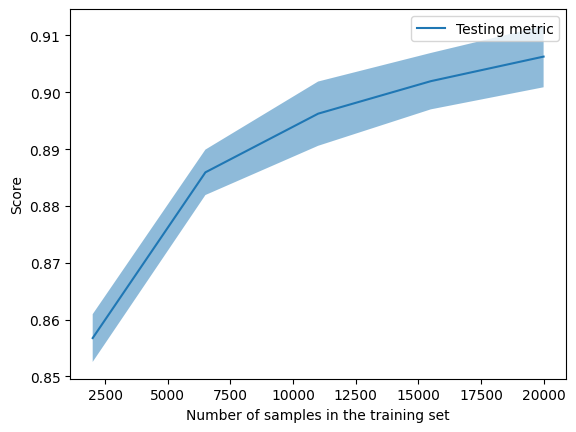
\includegraphics[scale=0.6]{images/loss.png}
\end{figure}

As mentioned before, some other architectures and workflows were investigated
before the current one. This was done through the \texttt{GridSearchCV} feature.
An example can be seen below on how to look for the best values for the \(C\)
parameter and the n-gram range.

\begin{minted}[breaklines]{python}
    pipe = make_pipeline(TfidfVectorizer(min_df=5), LogisticRegression())
    param_grid = {"logisticregression__C": [0.001, 0.01, 0.1, 1, 10, 100],
    "tfidfvectorizer__ngram_range": [(1, 1), (1, 2), (1, 3)]}
    grid = GridSearchCV(pipe, param_grid, cv=5)
    grid.fit(text_train, y_train)
    print("Best cross-validation score: {:.2f}".format(grid.best_score_))
    print("Best parameters:\n{}".format(grid.best_params_))
\end{minted}

A heatmap table of this grid can be observed in Figure \ref{fig:heat}.

\begin{figure}[h]
    \centering
    \caption{Heat map visualisation of GridSearchCV}
    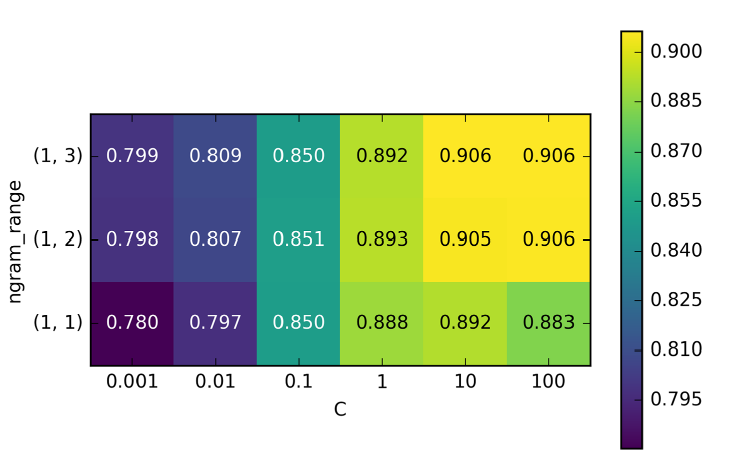
\includegraphics[scale=0.6]{images/heat.png}
    \label{fig:heat}
\end{figure}

\pagebreak

\section{Conclusion}

The development of this model shows that it is relatively easy to develop a
machine learning classifier thanks to the different Python packages and tools
available to the general public.
It was also found that a n-gram model performed better than a simple bag-of-words
vectorizer, since it provides the model with more context.
However, anything above tri-grams becomes too inefficient and achieves almost
no performance improvement.

Additionally, it was also found that past a certain point, it becomes quite
more difficult to achieve accuracy gains in a model without also increasing
processing time exponentially.
If a model with a higher accuracy than this one was desired, it would likely 
have to perform a higher degree of processing on the text, such as Natural
Language Processing, in order to have a better understanding of it and be able
to better classify the reviews.

\pagebreak

\printbibliography

\pagebreak

\appendix

\section{Classifier Source Code}

Also available as a
\href{https://colab.research.google.com/drive/14lITGB2M4x2nDNeRoziTfYY5tyL5PONz?usp=sharing}{Google Collab interactive demo}.

\subsection{Load Dataset}
First, load the dataset as it was downloaded or load from a cache.

\begin{minted}[breaklines]{python}
import pickle
from pathlib import Path

from sklearn.datasets import load_files


def load_files_and_pickle(data_dir: str , cache_path: Path):
    """Load dataset from cache if existent else load from original files and save cache."""
    dataset = None
    
    if cache_path.is_file():
        with cache_path.open("rb") as f:
            dataset = pickle.load(f)
    else:
        dataset = load_files(data_dir, categories=["pos", "neg"])
        
        with cache_path.open("wb") as f:
            pickle.dump(dataset, f)
    return dataset
            
        
reviews_train = load_files_and_pickle("aclImdb/train/", Path("acl_train_pickle"))
reviews_test = load_files_and_pickle("aclImdb/test/", Path("acl_test_pickle")) 
\end{minted}

\subsection{Filter HTML breakline tags}

The reviews are filtered to clear any HTML \texttt{<br>} tags, which the reviews still contain.

\begin{minted}[breaklines]{python}
train_text = [doc.replace(b"<br />", b" ") for doc in reviews_train.data]
test_text = [doc.replace(b"<br />", b" ") for doc in reviews_test.data]
# Alias these for later use
y_train = reviews_train.target
y_test = reviews_test.target
\end{minted}

\subsection{Create a pipeline with LogisticRegression}

In this step, a pipeline is created, which will first run the data through a TfidfVectorizer, which will extract n-grams from the reviews.
Then, the LogisticRegression algorithm will be trained with this data.

\begin{minted}[breaklines]{python}
import joblib
from sklearn.feature_extraction.text import TfidfVectorizer
from sklearn.linear_model import LogisticRegression
from sklearn.pipeline import make_pipeline

model_filename = "model.joblib"
ngram_range = (1, 3)
logreg_C = 10
logreg_max_iter = 500
\end{minted}

\begin{minted}[breaklines]{python}
if Path(model_filename).is_file():
    pipe = joblib.load(model_filename)
else:
    pipe = make_pipeline(
        TfidfVectorizer(ngram_range=ngram_range, min_df=5),
        LogisticRegression(max_iter=logreg_max_iter, solver='saga', C=logreg_C)
    )

    pipe.fit(train_text, y_train)
    joblib.dump(pipe, model_filename)

\end{minted}

\subsection{Test the model.}

\mint{python}|pipe.score(test_text, y_test)|


\end{document}
